\documentclass[a4paper]{article}

% Packages
\usepackage{geometry}
\geometry{left=1.5cm, right=1.5cm, top=2.54cm, bottom=2.54cm}
\usepackage{graphicx, setspace, amsmath, amssymb, titlesec, fancyhdr, multicol, parskip, indentfirst, etoolbox, caption, cite, xcolor}
\usepackage{listings}
\usepackage{url}
\usepackage{hyperref}
\usepackage{tikz}
\usetikzlibrary{arrows.meta, positioning, shapes.geometric, fit, backgrounds, calc}
\lstset{
  basicstyle=\ttfamily,
  breaklines=true,
  columns=flexible
}
% Title Formatting
\titleformat{\section}{\centering\large\scshape}{\thesection}{1em}{}
\titleformat{\subsection}{\normalsize\bfseries}{\thesubsection.}{1em}{}
\setstretch{1.0}
\setlength{\parskip}{6pt}
\titlespacing{\section}{0pt}{6pt}{6pt}
\titlespacing{\subsection}{0pt}{6pt}{6pt}
\titlespacing{\subsubsection}{0pt}{6pt}{6pt}
% Document Title
\title{
    \textbf{Coordena\c{c}\~ao Distribu\'ida de Agentes Aut\^onomos com Exclus\~ao M\'utua via Broker Pub/Sub}
}

\date{}
\captionsetup{labelfont={small,sc}, textfont={small,sc}}
% Section Numbering
\renewcommand{\thesection}{\Roman{section}.}
\renewcommand{\thesubsection}{\textit{\Alph{subsection}.}}
\renewcommand{\thesubsubsection}{\textit{\arabic{subsubsection}.}}
\renewcommand{\thetable}{\Roman{table}}
\renewcommand{\thefigure}{\Roman{figure}}

% Make titles italic
\titleformat{\subsection}{\normalfont\large\itshape}{\thesubsection}{1em}{}
\titleformat{\subsubsection}{\normalfont\itshape}{\thesubsubsection}{1em}{}

\setcounter{page}{1}

% Fancy Header Configuration
\pagestyle{fancy}
\fancyhf{}

% First Page Header
\fancypagestyle{firstpage}{
    \fancyhead[C]{
        \centering
        {\fontsize{14pt}{10pt}\selectfont
        \textbf{Universidade de S\~ao Paulo}\\[0.5em]
        \textbf{ACH2157 - Desenvolvimento de Sistemas de Informa\c{c}\~ao Distribu\'idos}}\\[0.2em]
        {\fontsize{8pt}{10pt}\selectfont
        \textbf{Prof. Doutor:} Jo\~ao Luiz Bernardes Junior \textbf{Ano:} 2\textsuperscript{o} Semestre/2025\
    }
  }
}

% Default Header for Other Pages
\fancyhead[C]{\textbf{Escola de Artes, Ci\^encias e Humanidades - Universidade de S\~ao Paulo}}
\begin{document}

\maketitle
\vspace{-1.5cm}
\thispagestyle{firstpage}

% Authors Block
\begin{multicols}{2}
    \centering
    \textbf{Isabelle da Silva Tobias}\\
            15525991 \\
            T04

    \textbf{Kevin Rodrigues Nunes}\\
            15676030\\
            T94

    \columnbreak

    \textbf{Kau\~a Lima de Souza}\\
            15674702\\
            T94

    \textbf{Victor Yodono}\\
            13829040\\
            T94


\end{multicols}

\singlespacing
\setlength{\parskip}{6pt}
\setlength{\parindent}{0.5cm}

\begin{multicols}{2}
\setlength{\columnsep}{0.5cm}

\noindent \textbf{\textit{Resumo---}} Este documento apresenta o planejamento e a arquitetura de um sistema distribu\'ido de carrinhos aut\^onomos que navegam em um grid $N \times N$ sem colis\~oes. O problema central \'e a coordena\c{c}\~ao descentralizada de acesso a recursos compartilhados --- as c\'elulas do grid --- sem a presen\c{c}a de um coordenador central. Para resolv\^e-lo, cada agente implementar\'a um \textbf{algoritmo de exclus\~ao m\'utua distribu\'ida} (a definir), utilizando rel\'ogios l\'ogicos para ordena\c{c}\~ao causal dos eventos e desempate de prioridade. Al\'em da movimenta\c{c}\~ao, o sistema utiliza um mecanismo de \textbf{elei\c{c}\~ao distribu\'ida} para determinar qual carrinho atender\'a cada novo pedido que surge no grid. A comunica\c{c}\~ao entre os agentes \'e realizada via um \textbf{broker pub/sub} (a definir), seguindo o padr\~ao \textit{publish/subscribe}. S\~ao detalhados os t\'opicos de comunica\c{c}\~ao, os componentes internos de cada agente, os fluxos de opera\c{c}\~ao com e sem conten\c{c}\~ao de recursos, e o protocolo de elei\c{c}\~ao para atribui\c{c}\~ao de pedidos.

\vspace{0.3em}
\noindent \textbf{Nota:} O broker pub/sub e o algoritmo de exclus\~ao m\'utua ainda ser\~ao definidos. A tabela abaixo lista os candidatos em avalia\c{c}\~ao:

\vspace{0.3em}
\noindent
\begin{minipage}{\columnwidth}
\centering
\begin{tabular}{|l|p{4.2cm}|}
\hline
\textbf{Decis\~ao} & \textbf{Candidatos} \\ \hline
Broker & MQTT (Mosquitto), RabbitMQ, Redis Pub/Sub, ZeroMQ \\ \hline
Exclus\~ao M\'utua & Ricart-Agrawala, Maekawa, Token Ring, Lamport \\ \hline
Rel\'ogio L\'ogico & Lamport, Vetorial \\ \hline
\end{tabular}
\end{minipage}
\vspace{0.3em}


\section{Introdu\c{c}\~ao}

O desenvolvimento de sistemas distribu\'idos apresenta desafios fundamentais relacionados \`a coordena\c{c}\~ao de processos concorrentes que competem por recursos compartilhados. Em particular, o problema da \textbf{exclus\~ao m\'utua distribu\'ida} --- garantir que apenas um processo acesse um recurso cr\'itico por vez, sem depend\^encia de um coordenador centralizado --- \'e um dos pilares cl\'assicos da \'area.

Este projeto prop\~oe uma implementa\c{c}\~ao pr\'atica desses conceitos atrav\'es de um sistema multi-agente: carrinhos aut\^onomos que navegam em um grid $N \times N$ e devem coordenar seus movimentos para evitar colis\~oes. Cada c\'elula do grid \'e tratada como um recurso compartilhado, e o acesso exclusivo a ela ser\'a garantido por um \textbf{algoritmo de exclus\~ao m\'utua distribu\'ida} (ainda a definir), com ordena\c{c}\~ao temporal fornecida por \textbf{rel\'ogios l\'ogicos}.

A comunica\c{c}\~ao entre os agentes ser\'a mediada por um \textbf{broker pub/sub} (ainda a definir), seguindo o padr\~ao \textit{publish/subscribe}. O broker atuar\'a como intermedi\'ario de mensagens, mas n\~ao participar\'a da l\'ogica de coordena\c{c}\~ao --- toda a intelig\^encia de decis\~ao \'e distribu\'ida entre os agentes.

Al\'em da coordena\c{c}\~ao de movimento, o sistema incorpora um mecanismo de \textbf{elei\c{c}\~ao distribu\'ida} para a atribui\c{c}\~ao de pedidos. Quando um novo pedido surge em uma c\'elula do grid, os carrinhos dispon\'iveis competem entre si atrav\'es de um processo de elei\c{c}\~ao: cada candidato publica sua oferta (baseada em crit\'erios como dist\^ancia ao pedido e carga atual), e o vencedor --- eleito de forma descentralizada --- assume a responsabilidade de atend\^e-lo. Esse mecanismo elimina a necessidade de um despachante central e garante distribui\c{c}\~ao aut\^onoma de tarefas entre os agentes.

\section{Funcionamento Geral}

O protocolo de movimenta\c{c}\~ao de cada carrinho segue um fluxo baseado em requisi\c{c}\~ao e concess\~ao de acesso exclusivo \`a c\'elula de destino:

\begin{enumerate}
    \item O carrinho determina a pr\'oxima c\'elula $[x, y]$ para a qual deseja se mover.
    \item Publica um \texttt{lock\_request} no t\'opico correspondente, incluindo seu \textit{timestamp} l\'ogico de Lamport.
    \item Os demais carrinhos avaliam a requisi\c{c}\~ao: concedem acesso imediato se n\~ao disputam a mesma c\'elula, ou cedem prioridade ao menor \textit{timestamp} (desempate pelo identificador do processo).
    \item Ao receber aprova\c{c}\~ao de todos os demais agentes, o carrinho ocupa a c\'elula e publica a libera\c{c}\~ao do lock.
\end{enumerate}

\section{Tecnologias}

A Tabela~\ref{tab:tecnologias} apresenta o \textit{stack} tecnol\'ogico adotado no projeto, selecionado com foco em compatibilidade com os conceitos de sistemas distribu\'idos estudados na disciplina.

\noindent
\begin{minipage}{\columnwidth}
\centering
\captionof{table}{Stack tecnol\'ogico do sistema distribu\'ido}
\label{tab:tecnologias}
\vspace{0.3em}
\begin{tabular}{|l|l|}
\hline
\textbf{Componente} & \textbf{Tecnologia} \\ \hline
Comunica\c{c}\~ao & Broker Pub/Sub (a definir) \\ \hline
Linguagem & A definir (Python ou Java) \\ \hline
Sincroniza\c{c}\~ao & Rel\'ogio L\'ogico (a definir) \\ \hline
Exclus\~ao M\'utua & Algoritmo distribu\'ido (a definir) \\ \hline
Elei\c{c}\~ao Distribu\'ida & Algoritmo baseado em m\'etrica (dist\^ancia/carga) \\ \hline
\end{tabular}
\end{minipage}

\section{Arquitetura do Sistema Distribu\'ido}

\subsection{T\'opicos do Broker}

A comunica\c{c}\~ao entre os agentes \'e estruturada hierarquicamente nos t\'opicos descritos na Tabela~\ref{tab:topicos}. Essa organiza\c{c}\~ao permite que cada carrinho se inscreva seletivamente nos t\'opicos relevantes, minimizando o tr\'afego desnecess\'ario. Os nomes s\~ao ilustrativos e ser\~ao adaptados ao broker escolhido.

\noindent
\begin{minipage}{\columnwidth}
\centering
\captionof{table}{Hierarquia de t\'opicos do broker}
\label{tab:topicos}
\vspace{0.3em}
\begin{tabular}{|l|p{3.5cm}|}
\hline
\textbf{T\'opico} & \textbf{Descri\c{c}\~ao} \\ \hline
\texttt{carrinhos/\{id\}/posicao} & Broadcast da posi\c{c}\~ao atual \\ \hline
\texttt{carrinhos/\{id\}/heartbeat} & Sinal de vida (detec\c{c}\~ao de falhas) \\ \hline
\texttt{grid/\{x\}/\{y\}/lock\_request} & Pedido de reserva de c\'elula \\ \hline
\texttt{grid/\{x\}/\{y\}/lock\_response} & Aprova\c{c}\~ao/nega\c{c}\~ao \\ \hline
\texttt{grid/\{x\}/\{y\}/lock\_release} & Libera\c{c}\~ao da c\'elula \\ \hline
\texttt{pedidos/novo} & Novo pedido publicado no grid \\ \hline
\texttt{pedidos/\{id\}/candidatura} & Candidatura de um carrinho ao pedido \\ \hline
\texttt{pedidos/\{id\}/eleito} & Resultado da elei\c{c}\~ao (vencedor) \\ \hline
\end{tabular}
\end{minipage}

\subsection{Componentes Internos de Cada Agente}

Cada carrinho \'e modelado como um agente aut\^onomo composto por cinco m\'odulos que cooperam internamente, conforme ilustrado na Figura~\ref{fig:componentes}.

\end{multicols}

% ====== DIAGRAMA DE COMPONENTES ======
\begin{figure}[!ht]
\centering
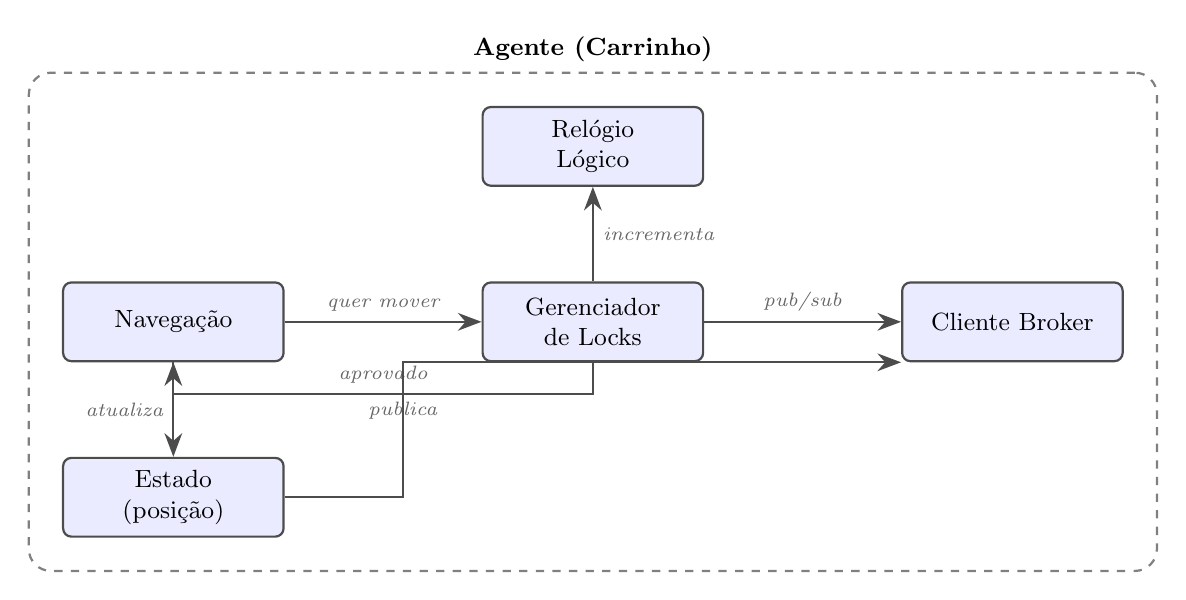
\begin{tikzpicture}[
    node distance=1.8cm and 2.5cm,
    block/.style={rectangle, draw=black!70, fill=blue!8, thick, minimum height=1cm, minimum width=2.8cm, align=center, rounded corners=3pt, font=\small},
    arr/.style={-{Stealth[length=3mm]}, thick, color=black!70},
    lbl/.style={font=\scriptsize\itshape, color=black!60}
]
    \node[block] (nav) {Navega\c{c}\~ao};
    \node[block, right=of nav] (lock) {Gerenciador\\de Locks};
    \node[block, right=of lock] (mqtt) {Cliente Broker};
    \node[block, above=1.2cm of lock] (lamp) {Rel\'ogio\\L\'ogico};
    \node[block, below=1.2cm of nav] (pos) {Estado\\(posi\c{c}\~ao)};

    \draw[arr] (nav) -- node[above, lbl] {quer mover} (lock);
    \draw[arr] (lock) -- node[above, lbl] {pub/sub} (mqtt);
    \draw[arr] (lock) -- node[right, lbl] {incrementa} (lamp);
    \draw[arr] (lock.south) -- ++(0,-0.4) -| node[near start, above, lbl] {aprovado} (nav.south);
    \draw[arr] (nav) -- node[left, lbl] {atualiza} (pos);
    \draw[arr] (pos.east) -- ++(1.5,0) |- node[near start, above, lbl] {publica} (mqtt.south west);

    % Bounding box
    \begin{scope}[on background layer]
        \node[draw=gray, dashed, thick, rounded corners=8pt, fit=(nav)(lock)(mqtt)(lamp)(pos), inner sep=12pt, label={[font=\small\bfseries]above:Agente (Carrinho)}] {};
    \end{scope}
\end{tikzpicture}
\caption{Diagrama de componentes internos de cada agente distribu\'ido}
\label{fig:componentes}
\end{figure}

\begin{multicols}{2}
\setlength{\columnsep}{0.5cm}

\begin{itemize}
    \item \textbf{Navega\c{c}\~ao:} determina o pr\'oximo movimento e solicita o lock da c\'elula de destino ao Gerenciador de Locks.
    \item \textbf{Gerenciador de Locks:} implementa o algoritmo de Ricart-Agrawala, gerenciando requisi\c{c}\~oes, filas de espera e respostas.
    \item \textbf{Rel\'ogio de Lamport:} mant\'em a ordena\c{c}\~ao causal dos eventos, incrementando o contador a cada evento local e atualizando-o ao receber mensagens externas.
    \item \textbf{Cliente Broker:} realiza \textit{publish} e \textit{subscribe} nos t\'opicos do broker.
    \item \textbf{Estado (posi\c{c}\~ao):} armazena e publica a posi\c{c}\~ao atual do carrinho.
\end{itemize}

\subsection{Fluxo Sem Conten\c{c}\~ao}

A Figura~\ref{fig:seq-normal} ilustra o cen\'ario em que n\~ao h\'a disputa pela mesma c\'elula. O Carrinho A solicita acesso \`a c\'elula $[2,3]$, recebe aprova\c{c}\~ao imediata e realiza o movimento.

\end{multicols}

% ====== DIAGRAMA DE SEQUENCIA - SEM CONFLITO ======
\begin{figure}[!ht]
\centering
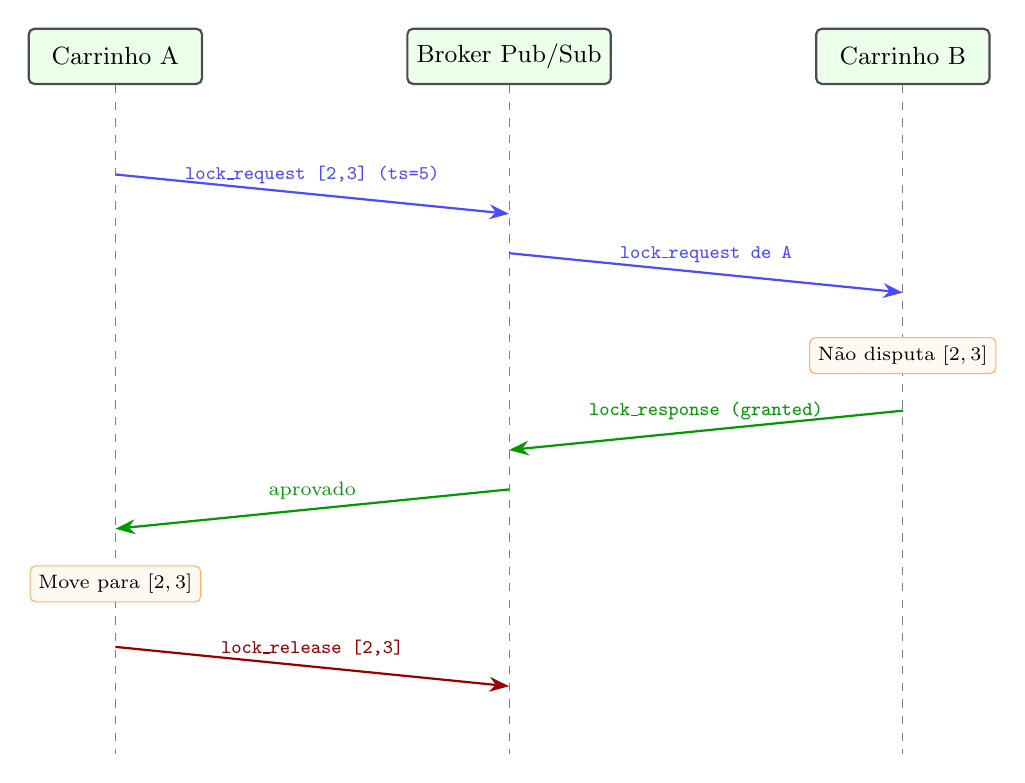
\begin{tikzpicture}[
    font=\small,
    actor/.style={rectangle, draw=black!70, fill=green!8, thick, minimum width=2.2cm, minimum height=0.7cm, rounded corners=2pt},
    msg/.style={-{Stealth[length=2.5mm]}, thick},
    note/.style={rectangle, draw=orange!60, fill=orange!5, rounded corners=2pt, font=\scriptsize, align=center, inner sep=3pt}
]
    % Actors
    \node[actor] (A) at (0,0) {Carrinho A};
    \node[actor] (broker) at (5,0) {Broker Pub/Sub};
    \node[actor] (B) at (10,0) {Carrinho B};

    % Lifelines
    \draw[dashed, gray] (A.south) -- ++(0,-8.5);
    \draw[dashed, gray] (broker.south) -- ++(0,-8.5);
    \draw[dashed, gray] (B.south) -- ++(0,-8.5);

    % Messages
    \draw[msg, blue!70] (0,-1.5) -- node[above, font=\scriptsize] {\texttt{lock\_request [2,3] (ts=5)}} (5,-2);
    \draw[msg, blue!70] (5,-2.5) -- node[above, font=\scriptsize] {\texttt{lock\_request de A}} (10,-3);

    \node[note] at (10,-3.8) {N\~ao disputa $[2,3]$};

    \draw[msg, green!60!black] (10,-4.5) -- node[above, font=\scriptsize] {\texttt{lock\_response (granted)}} (5,-5);
    \draw[msg, green!60!black] (5,-5.5) -- node[above, font=\scriptsize] {aprovado} (0,-6);

    \node[note] at (0,-6.7) {Move para $[2,3]$};

    \draw[msg, red!60!black] (0,-7.5) -- node[above, font=\scriptsize] {\texttt{lock\_release [2,3]}} (5,-8);
\end{tikzpicture}
\caption{Diagrama de sequ\^encia --- fluxo sem conten\c{c}\~ao de recursos}
\label{fig:seq-normal}
\end{figure}

\begin{multicols}{2}
\setlength{\columnsep}{0.5cm}

\subsection{Fluxo Com Conten\c{c}\~ao (Mesma C\'elula)}

Quando dois carrinhos disputam a mesma c\'elula simultaneamente, o algoritmo de exclus\~ao m\'utua resolve o conflito: o agente com menor \textit{timestamp} l\'ogico obt\'em prioridade. Em caso de empate, o menor identificador de processo vence. O agente preterido enfileira a requisi\c{c}\~ao e aguarda a libera\c{c}\~ao do recurso para tentar novamente. A Figura~\ref{fig:seq-conflito} ilustra esse cen\'ario.

\end{multicols}

% ====== DIAGRAMA DE SEQUENCIA - COM CONFLITO ======
\begin{figure}[!ht]
\centering
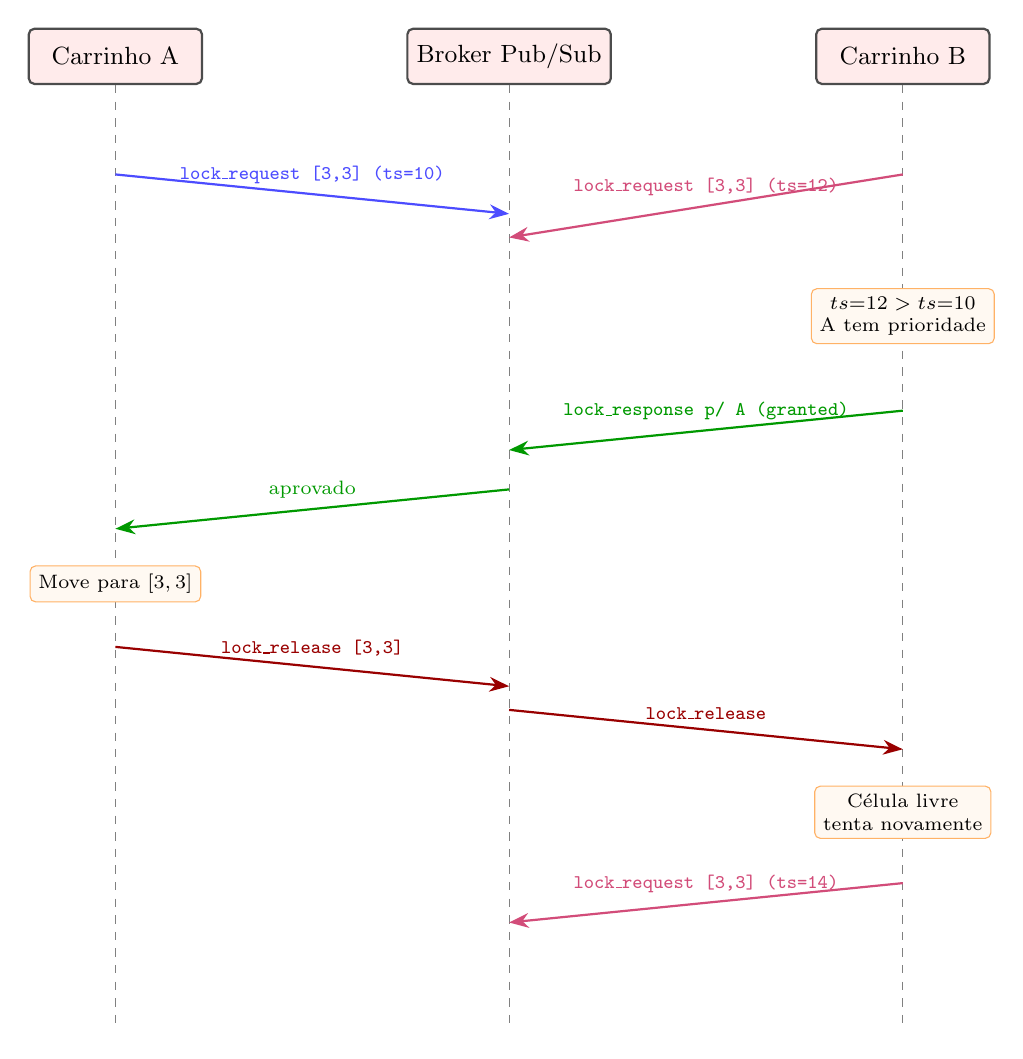
\begin{tikzpicture}[
    font=\small,
    actor/.style={rectangle, draw=black!70, fill=red!8, thick, minimum width=2.2cm, minimum height=0.7cm, rounded corners=2pt},
    msg/.style={-{Stealth[length=2.5mm]}, thick},
    note/.style={rectangle, draw=orange!60, fill=orange!5, rounded corners=2pt, font=\scriptsize, align=center, inner sep=3pt}
]
    % Actors
    \node[actor] (A) at (0,0) {Carrinho A};
    \node[actor] (broker) at (5,0) {Broker Pub/Sub};
    \node[actor] (B) at (10,0) {Carrinho B};

    % Lifelines
    \draw[dashed, gray] (A.south) -- ++(0,-12);
    \draw[dashed, gray] (broker.south) -- ++(0,-12);
    \draw[dashed, gray] (B.south) -- ++(0,-12);

    % Concurrent requests
    \draw[msg, blue!70] (0,-1.5) -- node[above, font=\scriptsize] {\texttt{lock\_request [3,3] (ts=10)}} (5,-2);
    \draw[msg, purple!70] (10,-1.5) -- node[above, font=\scriptsize] {\texttt{lock\_request [3,3] (ts=12)}} (5,-2.3);

    \node[note] at (10,-3.3) {$ts{=}12 > ts{=}10$\\A tem prioridade};

    % B grants to A
    \draw[msg, green!60!black] (10,-4.5) -- node[above, font=\scriptsize] {\texttt{lock\_response p/ A (granted)}} (5,-5);
    \draw[msg, green!60!black] (5,-5.5) -- node[above, font=\scriptsize] {aprovado} (0,-6);

    \node[note] at (0,-6.7) {Move para $[3,3]$};

    % A releases
    \draw[msg, red!60!black] (0,-7.5) -- node[above, font=\scriptsize] {\texttt{lock\_release [3,3]}} (5,-8);
    \draw[msg, red!60!black] (5,-8.3) -- node[above, font=\scriptsize] {\texttt{lock\_release}} (10,-8.8);

    \node[note] at (10,-9.6) {C\'elula livre\\tenta novamente};

    % B retries
    \draw[msg, purple!70] (10,-10.5) -- node[above, font=\scriptsize] {\texttt{lock\_request [3,3] (ts=14)}} (5,-11);
\end{tikzpicture}
\caption{Diagrama de sequ\^encia --- resolu\c{c}\~ao de conflito via exclus\~ao m\'utua distribu\'ida}
\label{fig:seq-conflito}
\end{figure}

% ====== SECAO DE ELEICAO ======
\begin{multicols}{2}
\setlength{\columnsep}{0.5cm}

\subsection{Elei\c{c}\~ao Distribu\'ida para Atribui\c{c}\~ao de Pedidos}

Al\'em da coordena\c{c}\~ao de movimento, o sistema precisa decidir \textbf{qual carrinho atender\'a cada pedido} que surge no grid. Essa decis\~ao \'e feita de forma totalmente descentralizada, sem um despachante central, atrav\'es de um processo de elei\c{c}\~ao distribu\'ida.

O fluxo de elei\c{c}\~ao funciona da seguinte maneira:

\begin{enumerate}
    \item Um novo pedido \'e publicado no t\'opico \texttt{pedidos/novo}, contendo a c\'elula de origem $[x, y]$ e um identificador \'unico.
    \item Cada carrinho dispon\'ivel calcula sua \textbf{m\'etrica de aptid\~ao} (por exemplo, dist\^ancia Manhattan at\'e o pedido, carga atual de tarefas, ou uma combina\c{c}\~ao ponderada de ambos).
    \item Cada candidato publica sua m\'etrica no t\'opico \texttt{pedidos/\{id\}/candidatura}, dentro de uma janela de tempo definida.
    \item Ap\'os a janela de candidatura, cada carrinho compara as m\'etricas recebidas. O agente com a \textbf{menor m\'etrica} (mais apto) vence a elei\c{c}\~ao. Em caso de empate, o menor identificador de processo desempata.
    \item O vencedor publica a confirma\c{c}\~ao no t\'opico \texttt{pedidos/\{id\}/eleito} e inicia a navega\c{c}\~ao at\'e a c\'elula do pedido.
\end{enumerate}

Esse mecanismo garante que a atribui\c{c}\~ao de tarefas \'e \textbf{aut\^onoma e distribu\'ida}: nenhum n\'o central decide quem atende o qu\^e. A Figura~\ref{fig:seq-eleicao} ilustra o fluxo de elei\c{c}\~ao entre tr\^es carrinhos.

\end{multicols}

% ====== DIAGRAMA DE SEQUENCIA - ELEICAO ======
\begin{figure}[!ht]
\centering
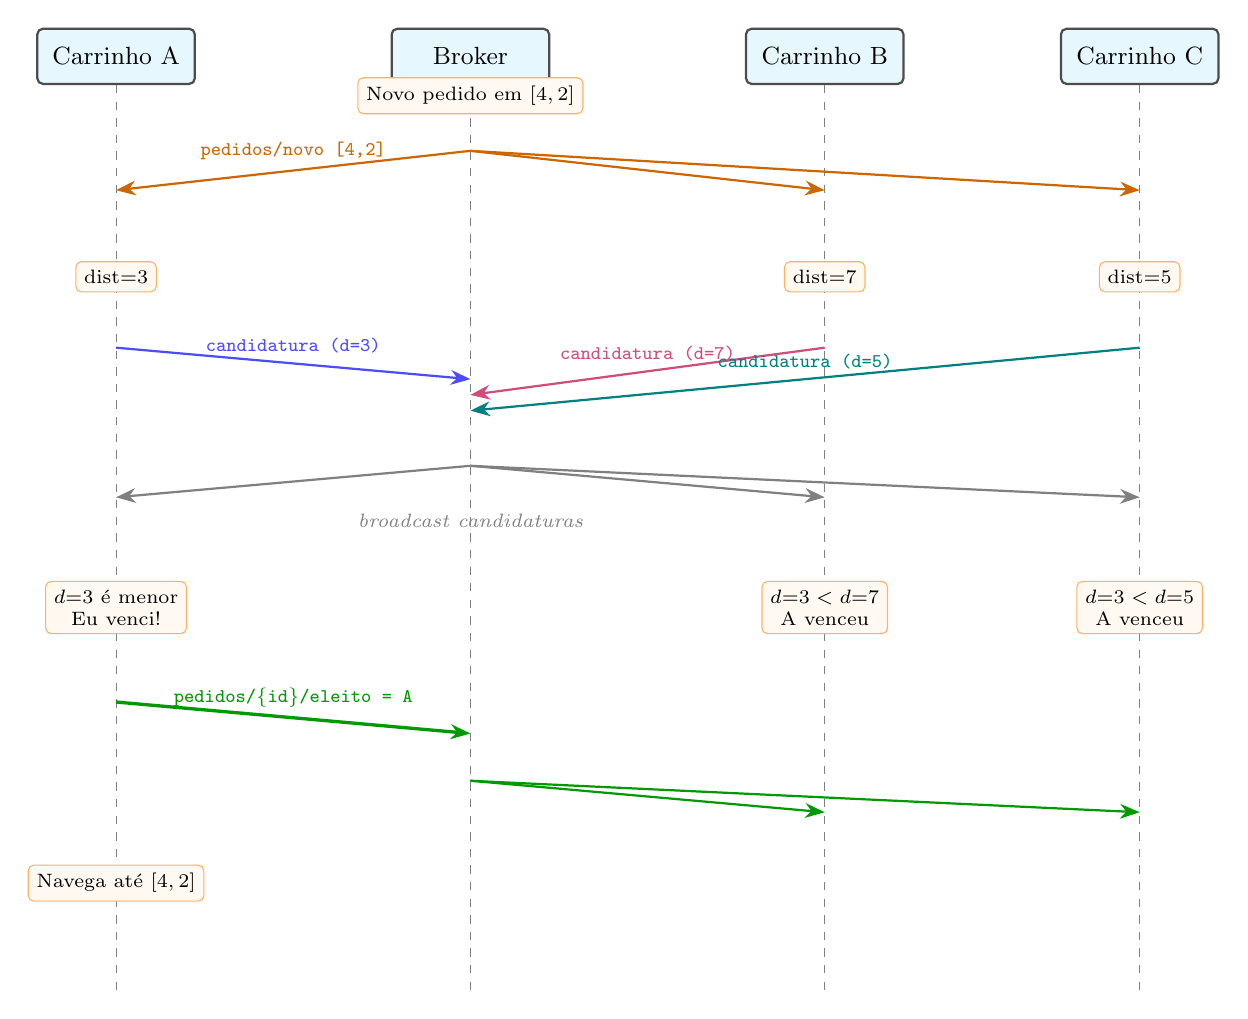
\begin{tikzpicture}[
    font=\small,
    actor/.style={rectangle, draw=black!70, fill=cyan!10, thick, minimum width=2cm, minimum height=0.7cm, rounded corners=2pt},
    msg/.style={-{Stealth[length=2.5mm]}, thick},
    note/.style={rectangle, draw=orange!60, fill=orange!5, rounded corners=2pt, font=\scriptsize, align=center, inner sep=3pt}
]
    % Actors
    \node[actor] (A) at (0,0) {Carrinho A};
    \node[actor] (broker) at (4.5,0) {Broker};
    \node[actor] (B) at (9,0) {Carrinho B};
    \node[actor] (C) at (13,0) {Carrinho C};

    % Lifelines
    \draw[dashed, gray] (A.south) -- ++(0,-11.5);
    \draw[dashed, gray] (broker.south) -- ++(0,-11.5);
    \draw[dashed, gray] (B.south) -- ++(0,-11.5);
    \draw[dashed, gray] (C.south) -- ++(0,-11.5);

    % New order
    \draw[msg, orange!80!black] (4.5,-1.2) -- node[above, font=\scriptsize] {\texttt{pedidos/novo [4,2]}} (0,-1.7);
    \draw[msg, orange!80!black] (4.5,-1.2) -- node[above, font=\scriptsize] {} (9,-1.7);
    \draw[msg, orange!80!black] (4.5,-1.2) -- node[above, font=\scriptsize] {} (13,-1.7);

    \node[note] at (4.5,-0.5) {Novo pedido em $[4,2]$};

    % Candidatures
    \node[note] at (0,-2.8) {dist=3};
    \node[note] at (9,-2.8) {dist=7};
    \node[note] at (13,-2.8) {dist=5};

    \draw[msg, blue!70] (0,-3.7) -- node[above, font=\scriptsize] {\texttt{candidatura (d=3)}} (4.5,-4.1);
    \draw[msg, purple!70] (9,-3.7) -- node[above, font=\scriptsize] {\texttt{candidatura (d=7)}} (4.5,-4.3);
    \draw[msg, teal] (13,-3.7) -- node[above, font=\scriptsize] {\texttt{candidatura (d=5)}} (4.5,-4.5);

    % Broadcast candidatures
    \draw[msg, gray] (4.5,-5.2) -- (0,-5.6);
    \draw[msg, gray] (4.5,-5.2) -- (9,-5.6);
    \draw[msg, gray] (4.5,-5.2) -- (13,-5.6);
    \node[font=\scriptsize\itshape, gray] at (4.5,-5.9) {broadcast candidaturas};

    % Each node evaluates
    \node[note] at (0,-7) {$d{=}3$ \'e menor\\Eu venci!};
    \node[note] at (9,-7) {$d{=}3 < d{=}7$\\A venceu};
    \node[note] at (13,-7) {$d{=}3 < d{=}5$\\A venceu};

    % Winner announces
    \draw[msg, green!60!black, line width=1.2pt] (0,-8.2) -- node[above, font=\scriptsize\bfseries] {\texttt{pedidos/\{id\}/eleito = A}} (4.5,-8.6);
    \draw[msg, green!60!black] (4.5,-9.2) -- (9,-9.6);
    \draw[msg, green!60!black] (4.5,-9.2) -- (13,-9.6);

    \node[note] at (0,-10.5) {Navega at\'e $[4,2]$};
\end{tikzpicture}
\caption{Diagrama de sequ\^encia --- elei\c{c}\~ao distribu\'ida para atribui\c{c}\~ao de pedido}
\label{fig:seq-eleicao}
\end{figure}

% ====== DIAGRAMA DE VISAO GERAL ======
\begin{figure}[!ht]
\centering
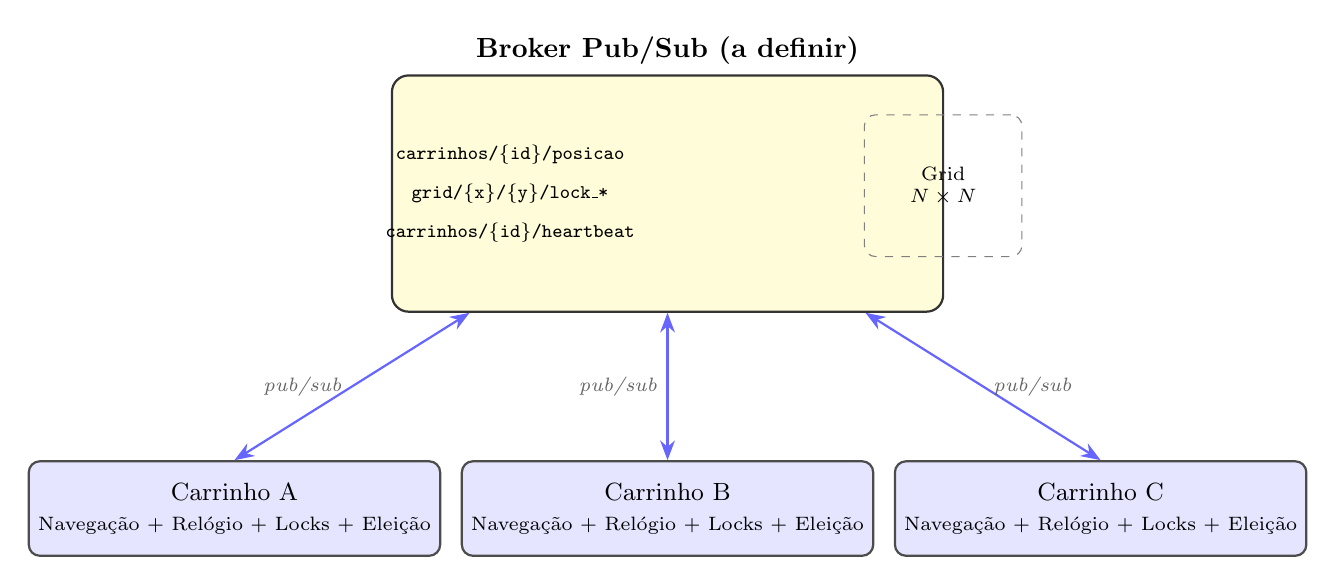
\begin{tikzpicture}[
    node distance=2cm,
    agent/.style={rectangle, draw=black!70, fill=blue!10, thick, minimum width=3cm, minimum height=1.2cm, align=center, rounded corners=4pt, font=\small},
    broker/.style={rectangle, draw=black!80, fill=yellow!15, thick, minimum width=7cm, minimum height=3cm, align=center, rounded corners=6pt},
    topic/.style={font=\scriptsize\ttfamily, align=center},
    conn/.style={{Stealth[length=2.5mm]}-{Stealth[length=2.5mm]}, thick, blue!60}
]
    % Broker
    \node[broker] (brk) at (0,0) {};
    \node[font=\bfseries, above] at (brk.north) {Broker Pub/Sub (a definir)};
    \node[topic] (t1) at (-2, 0.5) {carrinhos/\{id\}/posicao};
    \node[topic] (t2) at (-2, 0) {grid/\{x\}/\{y\}/lock\_*};
    \node[topic] (t3) at (-2,-0.5) {carrinhos/\{id\}/heartbeat};

    % Agents
    \node[agent] (ca) at (-5.5, -4) {Carrinho A\\{\scriptsize Navega\c{c}\~ao + Rel\'ogio + Locks + Elei\c{c}\~ao}};
    \node[agent] (cb) at (0, -4) {Carrinho B\\{\scriptsize Navega\c{c}\~ao + Rel\'ogio + Locks + Elei\c{c}\~ao}};
    \node[agent] (cc) at (5.5, -4) {Carrinho C\\{\scriptsize Navega\c{c}\~ao + Rel\'ogio + Locks + Elei\c{c}\~ao}};

    % Connections
    \draw[conn] (ca.north) -- node[left, font=\scriptsize\itshape, text=black!60] {pub/sub} ($(brk.south west)+(1,0)$);
    \draw[conn] (cb.north) -- node[left, font=\scriptsize\itshape, text=black!60] {pub/sub} (brk.south);
    \draw[conn] (cc.north) -- node[right, font=\scriptsize\itshape, text=black!60] {pub/sub} ($(brk.south east)+(-1,0)$);

    % N x N grid hint
    \node[draw=gray, dashed, rounded corners=4pt, minimum width=2cm, minimum height=1.8cm, align=center, font=\scriptsize] (grid) at (3.5, 0.1) {Grid\\$N \times N$};
\end{tikzpicture}
\caption{Vis\~ao geral da arquitetura distribu\'ida do sistema multi-agente}
\label{fig:visao-geral}
\end{figure}

\begin{multicols}{2}
\setlength{\columnsep}{0.5cm}

\subsection{Vis\~ao Geral}

A Figura~\ref{fig:visao-geral} apresenta a topologia geral do sistema. M\'ultiplos agentes (Carrinhos A, B, C, \ldots) comunicam-se exclusivamente atrav\'es do Broker MQTT central, seguindo o padr\~ao \textit{publish/subscribe}. \'E importante ressaltar que o Broker n\~ao exerce papel de coordena\c{c}\~ao: ele apenas roteia mensagens. Toda a l\'ogica de exclus\~ao m\'utua, ordena\c{c}\~ao causal, elei\c{c}\~ao de respons\'avel por pedidos e tomada de decis\~ao \'e inteiramente distribu\'ida entre os agentes, em conformidade com os princ\'ipios fundamentais de sistemas distribu\'idos.

O sistema garante as seguintes propriedades:
\begin{itemize}
    \item \textbf{Seguran\c{c}a (\textit{safety}):} no m\'aximo um carrinho ocupa cada c\'elula em qualquer instante.
    \item \textbf{Vivacidade (\textit{liveness}):} todo carrinho que solicita acesso a uma c\'elula eventualmente obt\'em permiss\~ao.
    \item \textbf{Ordena\c{c}\~ao causal:} os rel\'ogios de Lamport garantem uma ordena\c{c}\~ao total compat\'ivel com a causalidade dos eventos.
    \item \textbf{Distribui\c{c}\~ao aut\^onoma de tarefas:} o mecanismo de elei\c{c}\~ao garante que pedidos s\~ao atribu\'idos ao agente mais apto sem interven\c{c}\~ao central.
    \item \textbf{Detec\c{c}\~ao de falhas:} o mecanismo de \textit{heartbeat} permite identificar agentes inativos e evitar \textit{deadlocks}.
\end{itemize}

\end{multicols}
\end{document}
